\chapter{The Price of a Quantifier}\label{chap:quantifier}

In October 2026 a seventeen state, two symbol Turing machine appeared whose blank tape run beeps infinitely often if and only if the Collatz conjecture is true. This chapter reads that machine as a statement about the logical shape of the problem. As written, the conjecture is a $\Pi_2$\index{arithmetical hierarchy} sentence of arithmetic and the weak conjecture, that there are no nontrivial cycles, is $\Pi_1$. The difference is one quantifier, and the chapter is about what that quantifier costs: at most three states in this encoding, a heavy tail in its running time, and an a priori bound on the stopping time in any proof that lives in Peano arithmetic. Along the way the machine's clock turns out to be a quadratic functional of the orbit whose behaviour in the Bernoulli model is governed by the martingale of \cref{thm:martingale}, and in that model no function above the clock's per step cost is a supermartingale. We close with open problems.

\section{Busy beavers and Collatz}\label{sec:ch21:bb}

Rad\'o's\index{Busy Beaver function} Busy Beaver function $BB(n)$ is the largest number of steps an $n$ state two symbol Turing machine can run from a blank tape before halting. It is not computable, and its first few values are known only through a classification of every machine of the given size; $BB(5)=47{,}176{,}870$ was settled in 2024. The connection to Collatz was noticed early. Michel\index{Michel, P.}~\cite{michel1993} showed that the Marxen and Buntrock five state champion simulates the generalized Collatz function
\[
g(3m)=5m+6,\qquad g(3m+1)=5m+9,\qquad g(3m+2)=\uparrow,
\]
and that strong Busy Beaver candidates generally iterate something Collatz like; Aaronson's\index{Aaronson, S.} survey~\cite{aaronson2020} discusses why this may be structural. The six state holdouts Antihydra and Hydra are such objects, and their halting status is open because it is a Collatz like problem.

The Busy Beaver community calls a machine a cryptid\index{cryptid} when its blank tape behaviour is described completely by a simple arithmetic rule that is itself an open problem~\cite{bbchallengecryptids}. Cryptids were first noticed in the Beeping Busy Beaver variant, where a machine has no halt state but a designated beep state, and one asks whether it beeps only finitely often (quasihalts). Then the traffic reversed direction: instead of finding Collatz like rules inside small machines, people compiled specific open problems into small machines. The wiki~\cite{bbchallengecryptids} lists, among others, the Erd\H{o}s\index{Erdos, P.@Erd\H{o}s, P.} ternary conjecture in BB(15) (St\'erin and Woods~\cite{sterin2021}, 2021) and, from October 2026 and marked not independently verified, Goldbach's conjecture in BB(21) and the Riemann hypothesis in BB(95) (both credited to Google DeepMind). The weak Collatz conjecture is in BB(14), due to Charlie Reams~\cite{reams2026} and verified by Shawn Ligocki. The full Collatz conjecture is different in kind, and that is the subject of this chapter.

\section{The machine}\label{sec:ch21:machine}

\subsection{Statement}

Let $T_0$ and $T$ be the maps of \cref{def:maps}. The result below is from the Mira Cult repository~\cite{mira2026}; it has an ordinary proof and finite checks but no formal proof, and the wiki lists it as not independently verified. \Cref{sec:ch21:verify} reports our own check.

\begin{theorem}[Mira, 2026]\label{thm:ch21:mira}
There is a seventeen state, two symbol Turing machine with no halt transition and a designated beep state whose blank tape run beeps infinitely often if and only if every positive integer reaches $1$ under $T_0$. If the conjecture fails and $b$ is the least counterexample, the run emits exactly $b(b-1)/2$ beeps and is then silent forever.
\end{theorem}

The transition table is \cref{tab:ch21:tm}; the compact string, rows in alphabetical order with the read $0$ transition first, is
\begin{center}\footnotesize
\texttt{1RL0RB\_1LC1RB\_0LK0LD\_1RE1LD\_0RF0RB\_0LG0LG\_1LH1LG\_0RA0RI\_1RJ1RI\_}\\
\texttt{1RF1RF\_0RA1LK\_0LM0LM\_0LN1LM\_1RO1LN\_0RA0RP\_0RQ1RP\_1RL1RQ}
\end{center}
A beep is an exit from state $O$ on either read symbol.

\begin{table}[t]
\centering\footnotesize
\begin{tabular}{clll}
\toprule
State & Read 0 & Read 1 & Function \\
\midrule
A & 1RL & 0RB & Dispatch on whether the value is 1 \\
B & 1LC & 1RB & Find and fill the value hole \\
C & 0LK & 0LD & Move the hole left or detect the even meeting \\
D & 1RE & 1LD & Return to the halving marker \\
E & 0RF & 0RB & Move the marker right or detect the odd meeting \\
F & 0LG & 0LG & Place the odd step hole \\
G & 1LH & 1LG & Return to the odd step marker \\
H & 0RA & 0RI & Move that marker left or finish the odd step \\
I & 1RJ & 1RI & Find and fill the odd step hole \\
J & 1RF & 1RF & Advance the odd step hole \\
K & 0RA & 1LK & Return to the active field beginning \\
L & 0LM & 0LM & Place the reset or copy hole \\
M & 0LN & 1LM & Return over the active field to the separator \\
N & 1RO & 1LN & Increment the counter or restore a copy marker \\
O & 0RA & 0RP & Beep; finish the reset or copy another cell \\
P & 0RQ & 1RP & Cross the counter and separator \\
Q & 1RL & 1RQ & Find and advance the active field hole \\
\bottomrule
\end{tabular}
\caption{The seventeen state table. $A$ through $K$ are the arithmetic core, adapted from Reams's fourteen state weak Collatz machine; $L$ through $Q$ advance to the next input.}
\label{tab:ch21:tm}
\end{table}

\subsection{Representation}

A number is represented by the position of a missing one, the hole, inside a right hand block of ones. A separate unary counter on the left remembers which input is being tested. The configuration $C(n,v,W)$ has counter ones in cells $-n,\dots,-2$, a zero separator at $-1$, ones in cells $0,\dots,W-1$ except for a hole at $v-1$, zeros elsewhere, and the head at cell $0$ in state $A$. The blank tape is $C(1,1,1)$. The capacity $W$ is retained workspace, not a ceiling; extra ones to the right are never cleared and the field is extended when the trajectory grows.

The design decision that matters is the separation of the trajectory value from the starting input. A cycle search can abandon a trial as soon as the value exceeds its start, because a cycle that climbs above $n$ has a larger maximum, and the trial started at that maximum never exceeds its start; this is why Reams's weak Collatz machine needs no counter. The full conjecture cannot abandon anything, since a divergent orbit climbs forever. The input must survive arbitrarily large excursions, and that is what the left counter does.

\subsection{Three macro rules}

Writing $\to$ for the first return to state $A$ at cell $0$ after a positive finite number of transitions,
\begin{align*}
C(n,2k,W) &\to C(n,k,W), && \text{0 beeps},\\
C(n,2k+1,W) &\to C(n,3k+2,\max(W,3k+2)), && \text{0 beeps},\quad k\ge1,\\
C(n,1,W) &\to C(n+1,n+1,\max(W,n+1)), && n \text{ beeps}.
\end{align*}
The first two are one application of $T$. The third is the reset: increment the counter, copy its new length into the hole position, and beep $n$ times. The proofs are shuttle arguments. A marker and the hole move toward each other, and the parity of their meeting decides even or odd without a separate parity computation. In the odd case a second phase moves the hole two cells right for each cell the marker moves left, which is multiplication by three in this encoding. Each rule asserts equality of the whole tape, not merely of a decoded number.

\subsection{The clock}

Counting literal transitions gives exact running times,
\[
c(v)=\begin{cases} 2k(k+1), & v=2k,\\ 5k^2+9k+4, & v=2k+1>1,\end{cases}
\qquad R(n)=2n(n+2)
\]
for one arithmetic step on the value $v$ and for the reset from input $n$. These are independent of the capacity $W$, and
\begin{equation}\label{eq:ch21:cbound}
\tfrac12v^2\le c(v)\le2v^2\qquad(v\ge2).
\end{equation}
The quadratic form is not an artefact of clumsy encoding; it is unary arithmetic. A shuttle at marker to hole distance $d$ costs $2d+1$, and the distances shrink by two each shuttle, so the sum is quadratic in $v$. We write
\[
\tau(n)=\sum_{k=0}^{\sigma_\infty(n)-1} c\bigl(T^{(k)}(n)\bigr)
\]
for the time the machine spends on input $n$ before its reset, where $\sigma_\infty(n)$ is the total stopping time of $n$ under $T$.

\subsection{Theorem~\ref{thm:ch21:mira} from the macro rules}

The round for input $n$ iterates $T$ from $n$ until it hits $1$, beep free, then resets with $n$ beeps. If every orbit reaches $1$, infinitely many rounds complete and the run beeps infinitely often. If $b$ is the least input that does not reach $1$, rounds $1,\dots,b-1$ complete with $1+\dots+(b-1)=b(b-1)/2$ beeps, and round $b$ is an endless sequence of finite arithmetic macros, each of positive finite length by the formulas above, none of which visits $O$. This covers a nontrivial cycle and a divergent orbit alike, and the machine never needs a finite test for either. Finally $T$ and $T_0$ have the same reaches one predicate, since the value $3v+1\ge 4$ skipped by the shortcut is never $1$.

\section{Two conjectures, two quantifiers}\label{sec:ch21:quantifiers}

\subsection{$\Pi_1$ and $\Pi_2$}

The Collatz conjecture reads
\[
\forall n\ \exists k\ \ T^{(k)}(n)=1,
\]
a $\Pi_2$ sentence. A failure of it through a divergent orbit has no evident finite certificate: a divergent orbit is an infinite object and no finite prefix of it proves divergence. The weak conjecture reads
\[
\forall n\ \forall k\ge 1\ \ \bigl(T^{(k)}(n)=n \Rightarrow n\in\{1,2\}\bigr),
\]
a $\Pi_1$ sentence. Its failure has a finite certificate, a nontrivial cycle, and so it is equivalent to the non halting of an ordinary machine that searches for one. That is Reams's BB(14).

An ordinary Busy Beaver cryptid encodes a $\Pi_1$ statement: the machine halts iff the statement fails. There is no uniform way to encode a $\Pi_2$ statement as halting, but one can encode it as quasihalting:
\[
\text{Collatz true} \iff \text{infinitely many beeps} \iff \text{no quasihalt}.
\]
This is why the conjecture, in the form it is written, lives in BBB(17), and why it sits on the wiki beside the twin prime conjecture (BBB(18)) and the infinitude of Fermat primes (BBB(16)), which have the same form. The verification record up to $2^{71}$ (\cref{app:constants}) says, literally, that the machine run long enough emits at least $2^{71}(2^{71}+1)/2$ beeps. Finite computation can advance the beep count; no amount of it can rule out eventual silence.

\subsection{The collapse theorem}

The gap between the two sentences is an a priori bound. The conjecture itself says that $\sigma_\infty$ is finite everywhere, so a statement that assumes a bound on $\sigma_\infty$ has already assumed the conjecture. The content lies in the sentence one obtains from a bound that is merely proposed.

\begin{theorem}\label{thm:ch21:collapse}
Let $S:\N\to\N$ be computable and let $\Phi_S$ be the sentence $\forall n\ T^{(S(n))}(n)\in\{1,2\}$. Then:
\begin{enumerate}[label=(\roman*),leftmargin=2em]
\item $\Phi_S$ is $\Pi_1$. It is equivalent to the non halting of an ordinary Turing machine on blank tape, and by the MRDP theorem~\cite{matiyasevich1993} to the unsolvability in $\N$ of a single polynomial Diophantine equation.
\item $\Phi_S$ implies the Collatz conjecture.
\item If $\sigma_\infty(n)\le S(n)$ for every $n$ then $\Phi_S$ holds, and if $\Phi_S$ holds then $\sigma_\infty(n)\le S(n)+1$ for every $n$.
\end{enumerate}
\end{theorem}

\begin{proof}
The set $\{1,2\}$ is absorbing for $T$, since $T(1)=2$ and $T(2)=1$. The predicate $T^{(S(n))}(n)\in\{1,2\}$ is decidable uniformly in $n$ because $S$ is computable, so $\Phi_S$ is $\Pi_1$. A machine that enumerates $n$, computes $S(n)$, iterates $T$ that many times and halts if the result is outside $\{1,2\}$ halts iff $\Phi_S$ fails, and MRDP converts the halting problem of this fixed machine into a Diophantine equation. This is (i). For (ii) and the second half of (iii), an orbit in $\{1,2\}$ at step $S(n)$ is at $1$ by step $S(n)+1$. For the first half of (iii), an orbit at $1$ by step $S(n)$ stays in $\{1,2\}$.
\end{proof}

If Collatz is true then $\sigma_\infty$ is a total computable function, by running the orbit, and $\Phi_{\sigma_\infty}$ holds. What is missing is a bound one can write down in advance, with a proof that it is one. The difference between BBB(17) and some BB($m$) is such a bound, and so is the difference between a Lyapunov programme succeeding in its weak form (every orbit stops) and its strong form (every orbit stops by a computable time). The density theorems of \cref{chap:divergence,chap:backward}, including Tao's~\cite{tao2022} and Lau's~\cite{lau2026}, do not supply one.

\subsection{Provability}

A theorem going back to Kreisel, in the form given by Fairtlough and Wainer~\cite{fairtlough1998}, says that every function provably total in Peano arithmetic is bounded by some $H_\alpha$, $\alpha<\varepsilon_0$, in the Hardy hierarchy. If PA proves the Collatz conjecture then its Skolem function $\sigma_\infty$ is provably total and so $\sigma_\infty\le H_\alpha$ for some $\alpha<\varepsilon_0$. Contrapositively, if $\sigma_\infty$ is total and outgrows every $H_\alpha$ then the conjecture is true but unprovable in PA. Nobody expects this; the Lagarias and Weiss prediction of \cref{sec:ch21:stopping} is $\sigma_\infty(n)=O(\log n)$. But it shows that the $\Pi_2$ shape is not a formality. A proof in PA must produce, implicitly or explicitly, a bound, and the size of the bound places the proof in the hierarchy.

\subsection{The stopping time conjecture}\label{sec:ch21:stopping}

Lagarias and Weiss\index{Lagarias, J. C.}\index{Weiss, A.}~\cite{lagarias1992} analyse a branching random walk model and predict
\[
\limsup_{n\to\infty}\frac{\sigma_\infty(n)}{\log n}=\gamma_{BP}\approx 41.6776 .
\]
The constant counts steps of $T$. A path with a fraction $q$ of odd steps descends at rate $\log2-q\log3$ per step, and paths of this shape survive in the tree as long as $H(q)\ge q\log3$, with $H$ the entropy in nats; the boundary is $q\approx0.60909$, and $1/(\log2-q\log3)=41.677647$. Each odd step of $T$ is two steps of $T_0$, so the same model predicts about $(1+q)\,\gamma_{BP}\approx67.06$ for $T_0$. The typical slope is $\gamma_0\approx6.95$ for $T$; the record constant is larger because records are large deviations.

For an explicit $C$, the bound $S(n)=\lceil 42\log n\rceil+C$ is primitive recursive and \cref{thm:ch21:collapse} applies to it, so a stopping time conjecture with explicit constants is a $\Pi_1$ strengthening of Collatz, and it is a statement a halting machine can encode. The constant matters: the form ``there is a $C$ with $\sigma_\infty(n)\le42\log n+C$ for all $n$'' is $\Sigma_2$, and the $\limsup$ form does not supply $C$ either. \Cref{tab:ch21:records} shows the records to $10^6$. They stand well below the predicted constant in both counts, at $24.12$ against $41.68$ for $T$ and $38.42$ against $67.06$ for $T_0$ at $n=837{,}799$, as a $\limsup$ reached by large deviations should.

\begin{table}[t]
\centering
\begin{tabular}{rrrrr}
\toprule
$n$ & steps of $T$ & ratio to $\log n$ & steps of $T_0$ & ratio to $\log n$ \\
\midrule
3 & 5 & 4.55 & 7 & 6.37 \\
7 & 11 & 5.65 & 16 & 8.22 \\
9 & 13 & 5.92 & 19 & 8.65 \\
27 & 70 & 21.24 & 111 & 33.68 \\
230{,}631 & 278 & 22.51 & 442 & 35.79 \\
626{,}331 & 319 & 23.90 & 508 & 38.06 \\
837{,}799 & 329 & 24.12 & 524 & 38.42 \\
\bottomrule
\end{tabular}
\caption{Records of total stopping time over $\log n$ for $3\le n\le10^6$. The record holders are the same for $T$ and $T_0$ in this range.}
\label{tab:ch21:records}
\end{table}

Conceptually, one obtains a halting machine from Mira's by adding a budget: at the start of input $n$ write $S(n)$ in unary, decrement once per arithmetic macro, and halt if the budget runs out before the value enters $\{1,2\}$. Repeated halving, rounded up, of a copy of the counter gives $\lceil\log_2n\rceil$ in unary, so the budget that suits a small machine is dyadic, such as $S(n)=30\lceil\log_2n\rceil+C$, which is about $43.3\log n$ and still above the predicted constant. We do not give a state count. The point is that the states that implement the budget buy the inner quantifier.

\section{Is there an equation for Collatz?}\label{sec:ch21:equation}

The question was asked in the post that announced the machine~\cite{mira2026}. The two quantifier classes separate what is known from what is not.

\subsection{Cycles: yes}

By MRDP every $\Pi_1$ sentence is equivalent to the unsolvability of one polynomial equation, so there is a polynomial $P$ with
\[
\text{weak Collatz} \iff P(x_1,\dots,x_m)=0 \text{ has no solution in } \N^m .
\]
That is an abstract existence. The concrete equation is the cycle identity of \cref{sec:ch8:identity}, written in its sum form. A $T$ cycle with $k$ odd steps and $K$ steps in all, starting at $n$, satisfies
\[
n\,(2^{K}-3^{k}) = \sum_{j=0}^{k-1} 3^{k-1-j}\,2^{e_j},
\qquad 0\le e_0<e_1<\dots<e_{k-1}<K,
\]
an exponential Diophantine equation. Steiner's~\cite{steiner1977} theorem on circuits and the Simons and de Weger~\cite{simons2005} bounds on $m$ cycles proceed by Baker theory lower bounds on $|K\log 2-k\log 3|$ together with the continued fraction expansion of $\log_2 3$. For the cycle half of the problem there is an equation, and the state of the art is how well one can control it.

\subsection{The whole conjecture: not known}

As written, the whole conjecture has the form of a parametric family
\[
\forall n\ \exists \mathbf x\ \ Q(n,\mathbf x)=0
\]
each member of which must be solvable; here $Q(n,\mathbf x)=0$ says that the tuple $\mathbf x$ encodes a $T$ orbit from $n$ ending at $1$, and such a polynomial exists by MRDP. No single equation is known to be equivalent to it. Nothing rules one out: $\Pi_2$ is the form of the sentence, not a proved lower bound on the sentence itself, and a provable computable bound $S$ would give one by \cref{thm:ch21:collapse}. Whether divergence can have a finite certificate is similarly open; a proof that some orbit diverges would be one. Conway's~\cite{conway1972} theorem adds that for generalized Collatz maps the reaches one problem is undecidable, so whatever makes $3x+1$ provable, if it is provable, must be specific to $3x+1$.

\section{The clock in the Bernoulli model}\label{sec:ch21:clock}

We now study the clock in the Bernoulli model\index{Bernoulli model} of \cref{def:ch3:models}, where $x_{k+1}=\xi_{k+1}x_k$ with $\xi\in\{\tfrac12,\tfrac32\}$ with probability one half each and $x_0=n$. By \cref{thm:martingale} this is a nonnegative martingale, and by \cref{prop:absorb} it reaches $\nu=\inf\{k:x_k\le1\}$ (the $\tau$ of \cref{prop:absorb}) almost surely. In the spirit of \eqref{eq:ch21:cbound} we write
\[
\bar\tau(n)=\sum_{k<\nu}x_k^2,\qquad \bar t(n)=\sup_{k\le\nu}x_k
\]
for the model clock and the model excursion, so that \eqref{eq:ch21:cbound} gives a factor between $\tfrac12$ and $2$ term by term for integer orbits, and $\bar\tau$ is its model analogue.

\begin{theorem}\label{thm:ch21:tail}
There is a constant $C$ such that for every integer $n\ge2$ and every $x\ge1$,
\[
\frac{2(n-1)}{3n}\cdot\frac1{\sqrt x}\;\le\;\Prob\bigl(\bar\tau(n)\ge xn^2\bigr)\;\le\;\frac{C}{\sqrt x}.
\]
In particular $\E[\bar\tau(n)]=\infty$ for every $n\ge2$, and the family $\bar\tau(n)/n^2$, $n\ge2$, is tight, with medians bounded by a constant free of $n$.
\end{theorem}

\begin{proof}
Put $m=\sqrt x\,n\ge n$. For the lower bound, if $\bar t(n)\ge m$ then the excursion reaches $m$ at some $k<\nu$, so $\bar\tau(n)\ge m^2$. Stop the martingale at the first exit from $(1,m)$. It leaves below at a value at most $1$ and above at a value below $\tfrac32m$, so optional stopping gives $n\le1+\tfrac32m\,\Prob(\bar t(n)\ge m)$, whence $\Prob(\bar t(n)\ge m)\ge2(n-1)/(3m)$.

For the upper bound, \cref{prop:ch3:ville} gives $\Prob(\bar t(n)\ge m)\le n/m$. On the complement, $\bar\tau(n)\le\sum_{k\ge0}x_k^2\mathbf 1\{x_k<m\}$. Let $\mathbb Q$ be the measure with density $x_k/n$ on the first $k$ steps, under which the $\xi_i$ are independent with $\mathbb Q(\xi=\tfrac32)=\tfrac34$ and $\mathbb Q(\xi=\tfrac12)=\tfrac14$. Then $\E[x_k^2\mathbf 1\{x_k<m\}]=n\,\E_{\mathbb Q}[x_k\mathbf 1\{x_k<m\}]$. Under $\mathbb Q$ the walk $\log x_k$ has drift $\tfrac34\log\tfrac32-\tfrac14\log2>0$, so it is transient, and the expected number of visits to any interval of length $\log2$ is at most a constant $G$ that does not depend on the interval or the start (a renewal bound for a walk with positive drift). Splitting $(0,m)$ into the bands $[m2^{-j-1},m2^{-j})$, $j\ge0$,
\[
\E\Bigl[\sum_{k\ge0}x_k^2\mathbf 1\{x_k<m\}\Bigr]\le n\sum_{j\ge0}m2^{-j}G=2Gnm .
\]
Markov's inequality\index{Markov's inequality} gives $\Prob(\bar\tau(n)\ge m^2,\ \bar t(n)<m)\le2Gn/m$, and so $\Prob(\bar\tau(n)\ge m^2)\le(1+2G)n/m=(1+2G)/\sqrt x$. The mean is infinite because $\int^\infty y^{-1/2}\,dy$ diverges, and the uniform upper bound is tightness. Since $1+2G\ge1$ and $\Prob(\bar\tau(n)\ge xn^2)\le\tfrac12$ for $x\ge4(1+2G)^2$, the medians of $\bar\tau(n)/n^2$ are at most $4(1+2G)^2$.
\end{proof}

\begin{remark}\label{rem:ch21:perpetuity}
With the same factors $\xi_i$ for every $n$, the stopping time $\nu$ increases to infinity with $n$, so $\bar\tau(n)/n^2$ increases almost surely to $Y=\sum_{k\ge0}\xi_1^2\cdots\xi_k^2$, which is finite because $\log\xi$ has negative mean. This $Y$ is the perpetuity $Y\stackrel{d}{=}1+\xi^2Y$ with $\xi$ independent of $Y$. Since $\E[(\xi^2)^{1/2}]=1$, $\log\xi$ is non arithmetic and $\xi$ is bounded, the theorem of Kesten\index{Kesten, H.}~\cite{kesten1973} and Goldie\index{Goldie, C. M.}~\cite{goldie1991} gives $\Prob(Y>y)\sim c\,y^{-1/2}$ with $c>0$. So the limit law exists, and $\bar\tau(n)/n^2\le Y$ gives the upper bound of \cref{thm:ch21:tail} again, while its lower bound gives $\Prob(Y\ge x)\ge2/(3\sqrt x)$ for $x\ge1$, so $\tfrac23\le c\le1+2G$. The proof above is the elementary route: it uses the martingale of \cref{thm:martingale}, a change of measure and the visit bound of a transient walk.
\end{remark}

The tail has index $\tfrac12$ on the scale $n^2$ and the mean is infinite for every $n\ge2$, yet the family is tight. The mean is carried by rare, large excursions, as it is for the absorbed walk of \cref{sec:ch3:absorb}. For the deterministic orbits with $n\le10^6$ the fraction of $n$ with $t(n)\ge 10n$, $100n$, $1000n$ is $0.080$, $0.0076$, $0.00081$, where $t(n)$ is the maximal excursion of \cref{sec:ch3:ville}: about $0.8/L$ for $L=10,100,1000$, as \cref{prop:ch3:ville} leads one to expect.

\subsection{Empirical check}

For the deterministic orbits with $2\le n\le10^6$ the quantiles of $\tau(n)/n^2$ are $0.88$, $2.23$, $6.92$, $30.1$, $192$ at levels $0.10$, $0.25$, $0.50$, $0.75$, $0.90$, then $1.73\times10^4$ and $1.74\times10^6$ at $0.99$ and $0.999$; the mean is $1.07\times10^5$ and the maximum $6.9\times10^9$ at $n=270{,}271$. A least squares fit to the upper decile of the survival function gives tail index $0.513$ against the $\tfrac12$ of \cref{thm:ch21:tail} (\cref{fig:ch21:tail}). The fit steepens in the top $0.1$ percent, where the sample is thin and excursions meet the heuristic limit $\limsup\log t(n)/\log n=2$ of \cref{sec:ch3:ville}. The correlation of $\log(\tau(n)/n^2)$ with $\log(t(n)/n)^2$ is $0.976$.

\begin{figure}[t]
\centering
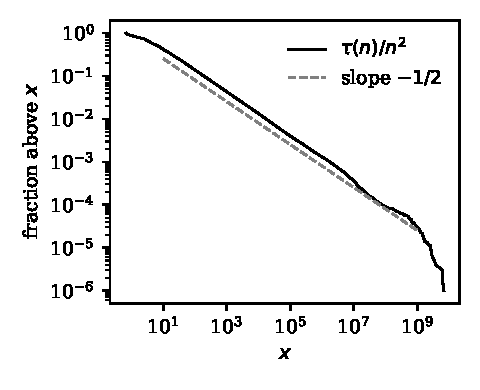
\includegraphics[width=0.48\textwidth]{figures/ch21_tail.pdf}\hfill
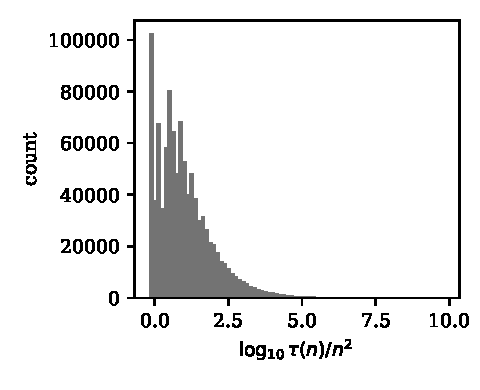
\includegraphics[width=0.48\textwidth]{figures/ch21_hist.pdf}
\caption{Left: survival function of $\tau(n)/n^2$, $n\le10^6$, with a line of slope one half. Right: histogram of $\log_{10}\tau(n)/n^2$.}
\label{fig:ch21:tail}
\end{figure}

The machine is therefore a correct but spectacularly slow Collatz verifier. Its total time through input $N$ is $\sum_{n\le N}(\tau(n)+R(n))$. The reset part is about $\tfrac23N^3$. The clock part is much larger: $3.17\times10^{22}$ at $N=10^6$, about $N^{3.75}$. Truncating the tail of \cref{thm:ch21:tail} at the same heuristic limit $t(n)\approx n^2$ suggests order $N^4$. Two hundred million transitions reach input $47$; input $27$ alone, whose orbit peaks at $4616$ under $T$, costs $60{,}537{,}762$.

\section{Which Lyapunov functions can work}\label{sec:ch21:lyapunov}

The majorizers of \cref{chap:lyapunov,chap:mmcollatz} are surrogates of the log potential, tangent at the current point. A different question is whether a function that bounds the clock's cost from above, at every value, could itself decrease in expectation and so serve as a Lyapunov function in the model. It cannot.

\begin{proposition}\label{prop:ch21:nomaj}
In the Bernoulli model there is no nonnegative function $F$ with $F(x)\ge\tfrac12x^2$ for all $x>1$ for which $(F(x_{k\wedge\nu}))_k$ is a supermartingale from some start $x_0=n\ge2$.
\end{proposition}

\begin{proof}
For a nonnegative supermartingale Ville's inequality gives $\Prob(\sup_kF(x_{k\wedge\nu})\ge\lambda)\le F(n)/\lambda$. If $\bar t(n)\ge m>1$ then $F$ reaches $\tfrac12m^2$, so $\Prob(\bar t(n)\ge m)\le2F(n)/m^2$. This contradicts the lower bound $2(n-1)/(3m)$ from the proof of \cref{thm:ch21:tail} for large $m$. The same proof excludes every $F\ge c\,x^p$ with $c>0$ and $p>1$.
\end{proof}

Powers show where the line falls. Let $\rho(p)=\E\xi^p=\tfrac12\bigl(2^{-p}+(3/2)^p\bigr)$. Then $\rho(0)=\rho(1)=1$ and $\rho$ is strictly convex, so $\rho<1$ on $(0,1)$ and $\rho>1$ on $(1,\infty)$. The minimum is the one of \cref{sec:ch3:lyapunov} and of the Chernoff rate $D$ in \cref{thm:density}:
\[
p^\ast=\frac{\log\bigl(\log2/\log\tfrac32\bigr)}{\log 3}\approx0.4881,\qquad\rho(p^\ast)\approx0.9659.
\]
So $V(v)=v^{p^\ast}$ contracts in expectation by about $3.4$ percent per step of the multiplicative model. For the actual odd branch $(3v+1)/2$ the added $\tfrac12$ works against the contraction: the one step factor $\tfrac12\bigl(2^{-p^\ast}+((3v+1)/(2v))^{p^\ast}\bigr)$ is $1.058$ at $v=1$, $1.014$ at $v=2$, $0.998$ at $v=3$, and decreases to $0.9659$ as $v\to\infty$ (the formula applies the odd branch at every $v$, as the model does). So the contraction holds for $v\ge3$ and is not uniform.

The clock measures work, and work in unary arithmetic is quadratic in the value; progress toward $1$ is measured by a concave power of the value. The balance condition $3^{p^\ast}=\log2/\log\tfrac32=1/(\log_23-1)$ is one more appearance of $\log_23$ from \cref{chap:cycles}; both are statements about how a halving competes with a tripling.

\section{Verification as a worked example}\label{sec:ch21:verify}

The construction is checked by its author with Python and C++ programs and an ordinary proof; it is not Lean or Rocq certified. We wrote a separate simulator from the transition string and the stated conventions alone and ran two checks. For every $1\le n\le60$, $1\le v\le400$ and $W\in\{v,\dots,v+3\}$ the machine was started in $C(n,v,W)$ and run to its first return to $A$ at cell $0$; in all $96{,}000$ cases the whole tape, the transition count and the beep count agree with the macro rules and the closed forms. Running $2\times10^8$ transitions from the blank tape gives $1{,}081$ beeps, the last at transition $181{,}892{,}196$. The closed forms predict completion of input $46$ at
\[
\sum_{n=1}^{46}\bigl(\tau(n)+R(n)\bigr)=181{,}892{,}196,
\]
and predict that in the orbit of $47$ the macro producing $3644$ from $2429$ ends at transition $198{,}095{,}814$, which is to the step the checkpoint the author reports with last value $3644$. So the author's run, our run and the closed forms agree exactly. This is a finite check of the macro rules, not a proof of them. The programs are listed in \cref{app:code}.

What remains for a formal proof is three lemmas by induction on the shuttle index, each asserting equality of whole tapes, and a global composition. Reams's weak Collatz machine has a formal proof upstream, so the work is to port the arithmetic core with its modified transitions and add the six state routine. We regard this as feasible and leave it as a project.

\section{Open problems}\label{sec:ch21:open}

\begin{problem*}[Q1. Minimality]\designation{Q1}\label{prob:ch21:minimal}
Is seventeen states minimal for a beeping machine equivalent to the full Collatz conjecture? There are $(4\cdot17)^{34}$ tables for a fixed beep state, and minimality is a statement about all smaller machines, including other cryptids. Structurally the full conjecture needs a separator, an increment and a copy that the cycle search does not, and the accounting $14-3+6=17$ relative to Reams's machine is explanatory rather than a proof. We conjecture the three state difference is close to the intrinsic price of the $\Pi_2$ quantifier in this encoding, and would be surprised by thirteen.
\end{problem*}

\begin{problem*}[Q2. A halting machine under the stopping time conjecture]\designation{Q2}\label{prob:ch21:halting}
Give an explicit BB($m$) machine, with a formal proof, that halts iff $\Phi_S$ fails for $S(n)=30\lceil\log_2n\rceil+C$ with an explicit $C$, by adding a logarithmic budget to the arithmetic core.
\end{problem*}

\begin{problem*}[Q3. The clock]\designation{Q3}\label{prob:ch21:clock}
Give explicit constants in \cref{thm:ch21:tail} and the constant $c$ of \cref{rem:ch21:perpetuity}. Does the deterministic $\tau(n)/n^2$ have the same tail, and is the empirical index $0.513$ converging to $\tfrac12$?
\end{problem*}

\begin{problem*}[Q4. Deterministic excursions]\designation{Q4}\label{prob:ch21:excursions}
\Cref{prop:ch3:ville} is a statement about the model. Is there a deterministic density version, that the set of $n\le N$ with $t(n)\ge Ln$ has size at most $CN/L$, and does it follow from the methods of \cref{chap:backward}?
\end{problem*}

\begin{problem*}[Q5. Binary encodings]\designation{Q5}\label{prob:ch21:binary}
A binary encoding of the value would make the clock $O(\log v)$ per step at the cost of many more states. Where is the state count at which the clock changes from quadratic to logarithmic, and does the tail of the clock then become light?
\end{problem*}
